\documentclass[12pt]{article}
\usepackage[T1]{fontenc}
\usepackage[letterpaper, margin=1in]{geometry}
\usepackage{graphicx}
\usepackage{caption}
\usepackage{placeins}
\usepackage{float}
\usepackage[noadjust]{cite}
\usepackage{etoolbox}
\usepackage{array}
\usepackage{ragged2e}
\usepackage{booktabs}
\usepackage{tabularx}
\usepackage[hyphens]{url}
\usepackage{amsmath}
\usepackage{amssymb}
\usepackage{enumitem}
\usepackage{setspace}
\usepackage{titlesec}
\usepackage[hidelinks]{hyperref}
% Load microtype after hyperref to avoid the ``Command \showhyphens has changed'' warning.
\usepackage{microtype}

% After hyperref loads, ensure IEEE-style centered REFERENCES heading (article \thebibliography).
\AtBeginDocument{%
  \makeatletter
  \patchcmd{\thebibliography}{\section*{\refname}}{\par\section*{\centering\bfseries\refname}\vspace{0.25\baselineskip}}{}{}%
  \makeatother
}

% Half of prior stretch (was 1.78); for single-spacing use \singlespacing instead.
\setstretch{0.89}

\captionsetup{font=small,labelfont=bf,labelsep=period,skip=6pt}
\captionsetup[figure]{position=bottom}

\setlength{\parindent}{0.5in}
\setlength{\parskip}{0pt}
\setlength{\emergencystretch}{2em}

\titlespacing*{\section}{0pt}{18pt plus 2pt minus 1pt}{10pt plus 2pt minus 1pt}
\titlespacing*{\subsection}{0pt}{14pt plus 2pt minus 1pt}{8pt plus 1pt minus 1pt}
\titlespacing*{\subsubsection}{0pt}{10pt plus 2pt minus 1pt}{5pt plus 1pt}
\titleformat{\section}[block]{\normalfont\normalsize\bfseries}{\thesection.\hspace{0.5em}}{0pt}{\raggedright}
\titleformat{\subsection}[block]{\normalfont\normalsize\bfseries}{\thesubsection.\hspace{0.5em}}{0pt}{\raggedright}
\titleformat{\subsubsection}[block]{\normalfont\normalsize\bfseries}{\thesubsubsection.\hspace{0.5em}}{0pt}{\raggedright}

\setlist[itemize]{leftmargin=0.5in, labelsep=0.5em, itemsep=4pt, topsep=0.75\baselineskip, parsep=0pt, partopsep=0pt}
\setlist[itemize,2]{leftmargin=0.65in, itemsep=2pt, topsep=0.35\baselineskip, parsep=0pt, partopsep=0pt}
\setlist[enumerate]{leftmargin=0.5in, labelsep=0.5em, itemsep=4pt, topsep=0.75\baselineskip, parsep=0pt, partopsep=0pt}

\widowpenalty=10000
\clubpenalty=10000
\raggedbottom

\AtBeginEnvironment{thebibliography}{%
  \setlength{\itemsep}{1.5pt plus 0.5pt minus 0.5pt}%
  \setlength{\parsep}{0pt}%
  \setlength{\topsep}{6pt}%
}

\renewcommand{\arraystretch}{1.4}
\setlength{\abovedisplayskip}{12pt plus 4pt minus 3pt}
\setlength{\belowdisplayskip}{12pt plus 4pt minus 3pt}

\begin{document}
\hypersetup{pageanchor=false}
\pagenumbering{gobble}

\begin{titlepage}
\thispagestyle{empty}
\centering
\begin{spacing}{1.0}
\vspace*{0.5in}

{\large\bfseries Florida Polytechnic University\par}
\vspace{0.35em}
{\normalsize Department of Computer Science\par}

\vspace{0.45in}

\includegraphics[width=0.15\textwidth,keepaspectratio]{Figures/FloridaPolytechnicImage.png}

\vspace{0.5in}
{\normalsize Master's Thesis Proposal\par}

\vspace{0.55in}
{\large\bfseries\linespread{1}\selectfont
ROADFM-LITE: A SELF-SUPERVISED FOUNDATION MODEL FOR\\
ROAD-NETWORK-GROUNDED TRAJECTORY REPRESENTATION\\
WITH APPLICATION TO SYBIL ATTACK DETECTION\par}

\vspace{0.55in}
{\large\bfseries Bibek Gupta\par}
\vspace{0.25in}
{\normalsize Master of Science in Computer Science\par}
\vspace{0.2in}
{\normalsize April 2026\par}
\vspace{0.25in}
{\normalsize Time frame: August 2026 - April 2027\par}

\vfill

\begin{minipage}{0.88\textwidth}
\centering
\textbf{Advisor}\\[0.4em]
{\normalsize Dr.\ Ayesha Dina and Dr.\ Luis Jaimes}

\vspace{0.8em}
\textbf{Member(s)}\\[0.35em]
{\normalsize Dr.\ Ayesha Dina, Dr.\ Luis Jaimes\\[0.35em]
Dr.\ Chamat Gunawardena, Dr.\ Sanjeeta N.~Ghimire}
\end{minipage}

\vspace{0.55in}
\end{spacing}
\end{titlepage}

\clearpage
\hypersetup{pageanchor=true}
\setcounter{page}{1}
\pagenumbering{arabic}

\begin{center}
\vspace*{0.25in}
{\bfseries ABSTRACT}\\[\baselineskip]
\end{center}
\vspace{\baselineskip}
\begingroup
\setlength{\parskip}{0.35em plus 0.08em minus 0.05em}
\setlength{\parindent}{0pt}
\justifying
Vehicular crowdsensing systems are increasingly vulnerable to Sybil attacks, in which a single adversary forges multiple vehicle identities to inject fabricated Basic Safety Messages and claim illegitimate rewards. These attacks are difficult to detect because forged messages can appear locally plausible in position, speed, and heading while concealing their illegitimacy in temporal inconsistencies, replay behavior, and physically unrealistic motion patterns that only emerge over longer observation windows. Existing detection methods either rely on hand-crafted kinematic features that generalize poorly across traffic conditions, or require large quantities of labeled attack data that are expensive to obtain and unlikely to cover novel adversarial strategies.

This thesis proposes RoadFM-Lite, a self-supervised foundation model that addresses these limitations by learning road-network-grounded trajectory representations directly from vehicular message traces without requiring labeled attack samples at pretraining time. RoadFM-Lite operates through two complementary pretraining objectives: masked trajectory reconstruction (MTR), which captures normal short-horizon motion regularities, and trajectory consistency prediction (TCP), which trains the model to recognize synthetic perturbations including replay, shuffling, speed-scaling, and positional offsets. Because the training data is generated by SUMO, a microscopic traffic simulator operating on a real urban road network, the learned representations implicitly encode lane-following behavior, intersection dynamics, and network-constrained motion without requiring an explicit road graph or map-matching pipeline.

The pretrained model is evaluated under three paradigms: few-shot contrastive fine-tuning with limited labeled examples, zero-shot retrieval-based detection using a benign memory bank, and scenario-holdout generalization across unseen traffic conditions and attack realizations. Comparisons against a from-scratch encoder, a feature-engineered Random Forest, and a supervised BiLSTM establish the value of self-supervised pretraining and the data efficiency of the resulting representations. This thesis demonstrates that road-network-grounded self-supervision provides a viable and practically scalable foundation for Sybil detection in settings where labeled data is scarce and attack variants are not known in advance.

\endgroup

\section{Motivation}\label{sec:motivation}

Vehicular crowdsensing (VCS) systems rely on networks of participating vehicles to collect traffic, environmental, and infrastructure data in exchange for monetary or service-based rewards \cite{wang2022imitation}. The economic incentive model that makes VCS viable also makes it an attractive target for Sybil attacks, in which a single adversary forges multiple fake vehicle identities to claim unearned rewards and inject corrupted data into the sensing pool \cite{douceur2002sybil}. Because every fabricated identity appears as a legitimate participant, Sybil attacks degrade both the economic integrity and the data quality of the entire crowdsensing ecosystem. Detecting these attacks therefore requires methods that can reliably distinguish fabricated vehicle trajectories from legitimate ones.

\subsection{Current Challenges}

Several critical challenges hinder effective Sybil detection in vehicular crowdsensing:

\begin{itemize}
    \item \textbf{Trajectory Plausibility:} Fabricated trajectories can look locally plausible in raw coordinate space. A forged trace may match realistic speed and heading ranges at individual time steps while still revealing replay artifacts, temporal discontinuities, or unrealistic motion changes over a longer sequence \cite{so2018integrating}.

    \item \textbf{Label Scarcity:} In real-world deployments, labeled Sybil attack samples are scarce. New attack variants emerge faster than ground-truth labels can be curated, making fully supervised detection approaches impractical. Detection systems must learn effective decision boundaries from very few labeled examples.

    \item \textbf{Scenario Generalization:} Vehicular datasets often contain multiple attack families and scenario groups that vary in traffic density, timing, and attack realization. A detector that memorizes a single split can fail when evaluated on another scenario from the same benchmark.

    \item \textbf{Representation Limitations:} Sybil detection in vehicular networks still relies heavily on hand-crafted plausibility rules, RSSI signals, trust scores, or fully supervised classifiers \cite{so2018integrating,yao2019multi,baza2022detecting,azam2022collaborative}. By contrast, self-supervised trajectory foundation models are designed to learn reusable motion representations from unlabeled sequences, but they have not been systematically adapted to vehicular message traces for Sybil detection.

    \item \textbf{Benchmark-to-Model Gap:} Raw vehicular message traces are message-oriented rather than model-ready. They must be transformed into trajectory windows, aligned by sender pseudonym and time, and split carefully to avoid leakage between nearly adjacent windows. This preprocessing problem is central to the study but is not addressed by off-the-shelf security baselines.
\end{itemize}

\subsection{Research Gap}

The core research gap addressed in this thesis is the absence of a self-supervised trajectory foundation model that learns road-network-grounded representations for Sybil detection in vehicular networks. Most existing studies either depend on hand-crafted heuristics or train directly on labeled attack data, while most trajectory foundation models are evaluated on generic mobility tasks rather than adversarial detection. Three practical gaps remain:

\begin{enumerate}
    \item \textbf{No benchmark-centered self-supervised pipeline.} There is no established method for converting raw vehicular message traces into reusable trajectory windows and learning sequence representations from them before downstream Sybil detection.

    \item \textbf{No few-shot or zero-shot focus.} Vehicular Sybil detection is still evaluated mostly in fully supervised settings, even though realistic deployments often begin with very few labeled attack samples.

    \item \textbf{No systematic within-benchmark generalization study.} Available vehicular security benchmarks contain multiple scenario families and time-group splits that allow evaluation beyond a single train/test split, but this structure is rarely used to measure whether learned representations transfer across scenario conditions.
\end{enumerate}

\subsection{Central Hypothesis}

Self-supervised pretraining on road-network-grounded vehicular trajectory windows using reconstruction and consistency objectives will produce foundation model embeddings that transfer more effectively to Sybil detection than training the same encoder architecture from scratch. This benefit should be largest in two settings where current methods are weakest: (1) few-shot supervision, where labeled attack examples are limited to 5 to 20 per class, and (2) scenario-holdout evaluation, where the detector is trained on one scenario group and tested on another.

The mechanistic claim is straightforward: a foundation model that has already learned how road-network-constrained vehicular trajectories evolve over time, and that has been trained to identify corrupted sequence patterns such as replay, shuffling, and offset perturbations, should separate benign and Sybil behavior more efficiently than a model that sees the same data only through supervised labels.

\subsection{Research Question}

\textbf{Does a self-supervised trajectory foundation model trained on road-network-grounded vehicular message traces produce representations that improve Sybil detection relative to supervised-only baselines, particularly under few-shot supervision and scenario-holdout evaluation?}

This question decomposes into four sub-questions:

\begin{enumerate}
    \item Does self-supervised pretraining improve Sybil detection accuracy compared to the same sequence encoder trained from scratch on the same data splits?

    \item Does the pretrained encoder improve label efficiency, i.e., require fewer labeled attack examples to reach a useful detection threshold?

    \item Does the pretrained encoder reduce performance loss when evaluation moves from one scenario group to another?

    \item Which components contribute most to downstream detection performance: masked reconstruction, trajectory consistency prediction, feature design, or context-window length?
\end{enumerate}

\subsection{Practical Significance}

The development of a self-supervised trajectory foundation model for road-network-grounded Sybil detection is practically important for four reasons:

\begin{itemize}
    \item \textbf{Deployment with Minimal Supervision:} A pretrained encoder that already captures motion regularities can be adapted with only a small labeled support set when new attack conditions appear.

    \item \textbf{Scenario Robustness:} If the model generalizes across different scenario groups, it is less likely to depend on a single curated split and more likely to capture durable behavioral signals.

    \item \textbf{Lightweight Foundation Model:} A single sequence encoder with compact pretraining heads is simpler to implement, train, and reproduce than multi-branch systems that require external maps or additional corpora, while still producing reusable road-network-grounded trajectory representations.

    \item \textbf{Reproducible Scope:} Building the foundation model on an established vehicular benchmark keeps the experimental scope focused and reproducible, and it makes the final pipeline and pretrained weights easier to release and reuse.
\end{itemize}

\subsection{Scientific Context}

This thesis sits at the intersection of three closely related research areas:

\begin{itemize}
    \item \textbf{Trajectory Self-Supervised Learning.}~Recent work has shown that masked modeling, contrastive learning, and related self-supervised objectives can produce reusable trajectory embeddings without manual annotation \cite{jiang2023start,chen2023self,lin2023pre}. The key open question for this thesis is whether those ideas can be adapted effectively to raw vehicular message traces.

    \item \textbf{Trajectory Anomaly and Consistency Modeling.}~Sequence models are increasingly used to learn what normal motion looks like and to detect corrupted or implausible temporal patterns \cite{chen2023self,jiang2023start}. This thesis draws on that idea by using synthetic trajectory corruptions during pretraining, but targets Sybil detection rather than generic anomaly detection.

    \item \textbf{Vehicular Sybil Detection.}~The vehicular security literature provides the attack framing, benchmark setting, and strong traditional baselines \cite{so2018integrating,yao2019multi,baza2022detecting,azam2022collaborative,zhou2011p2dap,van2018veremi,van2020veremi}. However, most of this literature still favors heuristics or fully supervised classifiers over reusable pretrained trajectory foundation models. This thesis targets that gap directly.
\end{itemize}

\section{Related Work}\label{sec:relatedwork}

The proposed research builds on recent work in trajectory foundation models, self-supervised representation learning, and vehicular security. This section emphasizes self-supervised sequence learning, road-network-grounded trajectory modeling, Sybil detection on vehicular benchmarks, and low-label evaluation settings.

\subsection{Trajectory Foundation Models}

Recent trajectory foundation models show that large-scale pretraining on unlabeled motion sequences can produce transferable embeddings for downstream mobility tasks. TrajFM \cite{lin2024trajfm} and UniTraj \cite{liang2025unitraj} are representative examples: both demonstrate that pretrained encoders can support region transfer and multiple downstream tasks when trained on large trajectory corpora. Their importance for this thesis is conceptual rather than direct. They establish that trajectory pretraining is useful, but they depend on large external corpora and are evaluated on generic mobility tasks such as prediction, retrieval, and similarity rather than adversarial detection.

For this thesis, the main lesson from these works is not to replicate their scale but to adapt the foundation model paradigm, that is, pretrain on unlabeled trajectory data and then adapt to downstream tasks, to a security-oriented vehicular setting. RoadFM-Lite shares this paradigm but applies it to road-network-grounded vehicular traces for Sybil detection rather than generic mobility analysis.

\subsection{Self-Supervised Trajectory Learning}

Self-supervised learning for trajectories has matured around several common pretraining strategies.

\textbf{Masked Modeling.} START \cite{jiang2023start} and related masked-trajectory methods learn useful motion representations by hiding part of a sequence and asking the encoder to reconstruct it.

\textbf{Contrastive and Multi-View Learning.} Contrastive self-supervised learning for large-scale trajectories \cite{chen2023self} and maximum multi-view entropy coding for trajectory embeddings \cite{lin2023pre} demonstrate that agreement across multiple views or augmentations can produce embeddings that transfer to downstream tasks.

These works are strong methodological priors for this thesis, but they are mostly optimized for generic trajectory semantics rather than Sybil-specific inconsistencies. In particular, they do not focus on replay behavior, local temporal reordering, or other corruption patterns that are especially relevant to fabricated vehicular messages. This is precisely where a security-oriented consistency objective becomes useful.

\subsection{Trajectory Anomaly and Consistency Modeling}

Trajectory anomaly detection is related to Sybil detection because both tasks require identifying motion patterns that deviate from normal behavior. Related lines of work show that temporal models can learn a notion of normality and then flag deviations \cite{jiang2023start,chen2023self}. However, Sybil behavior is not simply a generic outlier problem. A Sybil trajectory may be crafted to look locally plausible while still betraying replay artifacts, inconsistent timing, duplicated patterns, or systematic offsets over a window. That makes the task closer to sequence-consistency modeling than to unconstrained outlier detection. This thesis therefore borrows the idea of learning normal motion structure, but targets Sybil-specific corruptions generated directly from vehicular trajectory windows.

\subsection{Vehicular Sybil Detection and the VeReMi Benchmark}

The vehicular security literature provides the attack framing and the benchmark context for this study. VeReMi \cite{van2018veremi} and the VeReMi Extension \cite{van2020veremi} established a reusable benchmark for VANET misbehavior detection. On top of that benchmark, prior work has explored plausibility checks combined with machine learning \cite{so2018integrating}, RSSI-based methods \cite{yao2019multi}, proof-of-work and location-based methods \cite{baza2022detecting}, collaborative learning \cite{azam2022collaborative}, and pseudonym-based approaches such as P2DAP \cite{zhou2011p2dap}.

These methods are important baselines for the field, but they share two limitations that matter for this thesis. First, they usually operate with hand-crafted signals or directly supervised models rather than reusable pretrained sequence encoders. Second, they generally evaluate a detector on a fixed split instead of asking whether the representation remains useful under few-shot adaptation or scenario holdout. The VeReMi benchmark is therefore well established, but the representation-learning story on top of it is still underdeveloped.

\subsection{Few-Shot and Retrieval-Based Detection}

Few-shot adaptation and retrieval-based detection are standard tools in broader representation learning, but they are not yet common in vehicular Sybil detection. Supervised contrastive learning and related objectives make it possible to separate classes in embedding space with very limited labeled data \cite{chen2023self,lin2023pre}, which is attractive when attack labels are scarce. Likewise, a memory-bank or nearest-neighbor view of detection is useful when only benign reference behavior is available and explicit attack labels are limited.

These settings are especially relevant because they let the thesis evaluate not just raw classification accuracy, but also label efficiency and representation quality. In other words, the model should not only classify known attacks well; it should also adapt quickly and detect suspicious behavior when supervision is weak.

\subsection{Implicit Road-Network Grounding Through Simulation Data}

Several trajectory-learning papers achieve road-network grounding by consuming explicit map assets, road graphs, or external corpora \cite{mao2022jointly}. RoadFM-Lite takes a different approach: it achieves road-network-grounded representations implicitly because the VeReMi dataset is itself generated by SUMO, a microscopic traffic simulator that models vehicles on a real urban road network (the Luxembourg SUMO scenario). Every position, speed, heading, and acceleration value in VeReMi reflects road-constrained movement: vehicles follow lanes, decelerate at intersections, and turn according to the network topology.

This means the foundation model learns road-level structure from the trajectory data without requiring an explicit road graph as input. The approach is more reproducible, avoids dependencies on external map-matching pipelines, and keeps the experimental scope focused on the benchmark while still producing trajectory representations that are grounded in road-network dynamics.

\begin{figure}[H]
\centering
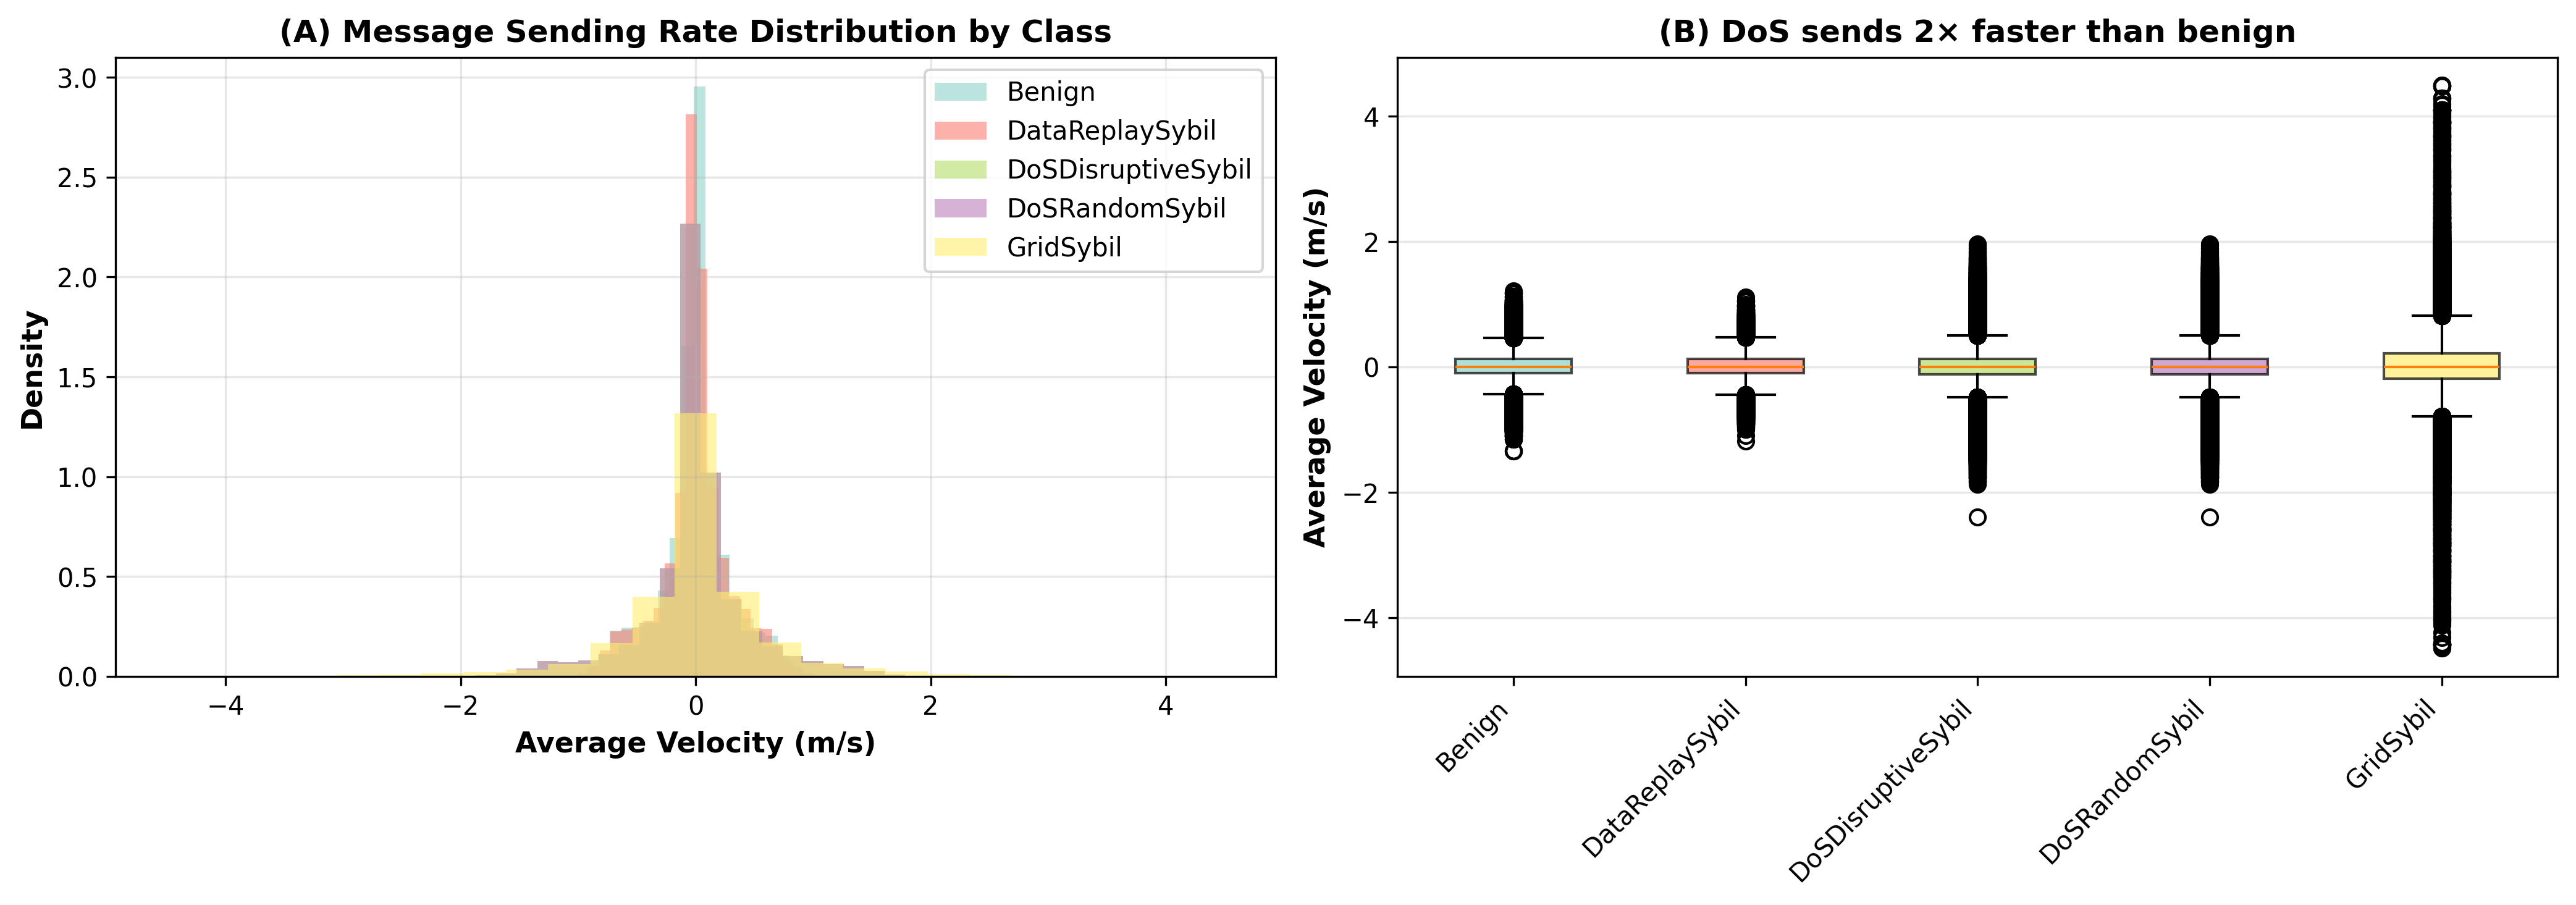
\includegraphics[width=0.64\textwidth]{Figures/PROPOSAL_2_temporal_discriminator.png}
\caption{Discriminative temporal feature: message sending rate. DoS attacks (e.g., A18, A19) can exhibit shorter inter-message intervals than benign traffic. (A) Histogram of inter-message gaps. (B) Boxplots by class. This pattern motivates trajectory consistency prediction (TCP) during pretraining.}
\label{fig:temporal_discriminator}
\end{figure}

\subsection{Research Gaps}

Our analysis of the literature reveals four concrete gaps that this thesis addresses:

\begin{enumerate}
    \item \textbf{Foundation Model Gap:} Sybil detection in vehicular networks still relies heavily on rule-based approaches, trust metrics, signal-based checks, or supervised classifiers \cite{so2018integrating,yao2019multi,baza2022detecting,azam2022collaborative}. Self-supervised trajectory foundation models that learn road-network-grounded representations for Sybil detection are largely absent.

    \item \textbf{Label-Efficiency Gap:} Few-shot contrastive adaptation and zero-shot retrieval are natural settings for security problems with scarce labels, but they are not standard practice in the vehicular Sybil literature.

    \item \textbf{Scenario-Generalization Gap:} Vehicular security datasets often contain multiple scenario families and group splits, yet this structure is rarely used to test whether learned representations transfer beyond one curated split.

    \item \textbf{Preprocessing Gap:} Raw vehicular message traces are typically message-oriented rather than model-ready. There is no widely adopted benchmark-centered pipeline for turning them into leakage-safe trajectory windows for self-supervised learning and downstream detection.
\end{enumerate}

\subsection{Our Contribution}

This thesis addresses those gaps through a focused and internally consistent contribution set. First, it proposes RoadFM-Lite as a self-supervised trajectory foundation model that learns road-network-grounded representations from simulated vehicular data. Second, it introduces a pretraining design based on masked trajectory reconstruction and trajectory consistency prediction using synthetic corruptions derived directly from the benchmark. Third, it evaluates the resulting embeddings under few-shot, zero-shot, fully supervised, and scenario-holdout settings, thereby measuring both label efficiency and within-benchmark generalization. Finally, it defines a reproducible preprocessing pipeline that converts raw vehicular messages into sender-aligned trajectory windows suitable for security-oriented sequence learning.

\section{Proposed Architecture}\label{sec:architecture}

The implementation of RoadFM-Lite follows an encoder-decoder foundation model design built directly on raw vehicular messages. The architecture has four components: a preprocessing stage that converts line-delimited traces into fixed-length trajectory windows, a Transformer encoder that produces road-network-grounded representations from those windows, a Transformer decoder that reconstructs masked or corrupted trajectory segments from the encoder representations, and task-specific heads that change across self-supervised pretraining and downstream detection. During pretraining, the encoder and decoder are trained jointly; during downstream Sybil detection, only the encoder is retained and the decoder is discarded, following the standard foundation model paradigm.

\subsection{Architectural Overview}

RoadFM-Lite achieves road-network-grounded trajectory representation without requiring an explicit road graph or map-matching pipeline as input. Because the VeReMi dataset is generated by the SUMO microscopic traffic simulator, every message trace already encodes road-constrained vehicle dynamics: position coordinates follow road geometry, speed profiles reflect network-level conditions, and heading changes correspond to turns and lane maneuvers. The foundation model learns from these inherently road-grounded fields---message time, sender identity fields, position, speed, acceleration, and heading---together with short-horizon deltas once windows are formed (Subsection~\ref{subsec:window}).

The end-to-end structure follows four conceptual blocks:

\begin{enumerate}[label=\textbf{(\arabic*)}, leftmargin=0.55in, labelsep=0.45em, itemsep=0.35\baselineskip, parsep=0pt, topsep=0.4\baselineskip, partopsep=0pt]

\item \textbf{Inputs.} Local VeReMi data comprise raw line-delimited JSON traces (including \texttt{sendTime}, sender and \texttt{senderPseudo}, \texttt{pos}, \texttt{spd}, \texttt{acl}, \texttt{hed}) and scenario folders with accompanying ground-truth traces.

\item \textbf{Preprocessing.} Messages are grouped by scenario and pseudonym, sorted by \texttt{sendTime}, mapped to per-message feature vectors with temporal deltas, and segmented into fixed-length windows (sliding or non-overlapping).

\item \textbf{Foundation model.} A Transformer encoder applies linear embedding, sinusoidal positional encoding, and stacked self-attention, then pools token states (mean or \texttt{CLS}) into a window-level representation. A Transformer decoder operates only during pretraining: mask-token queries with positional encoding attend to encoder states via cross-attention to reconstruct masked segments for MTR.

\item \textbf{Heads.} Reconstruction loss is computed from decoder outputs. Pooled encoder embeddings feed the TCP head during pretraining; after adaptation, they feed contrastive, linear classification, or nearest-neighbor retrieval heads for downstream Sybil evaluation.

\end{enumerate}

\begin{figure}[H]
\centering
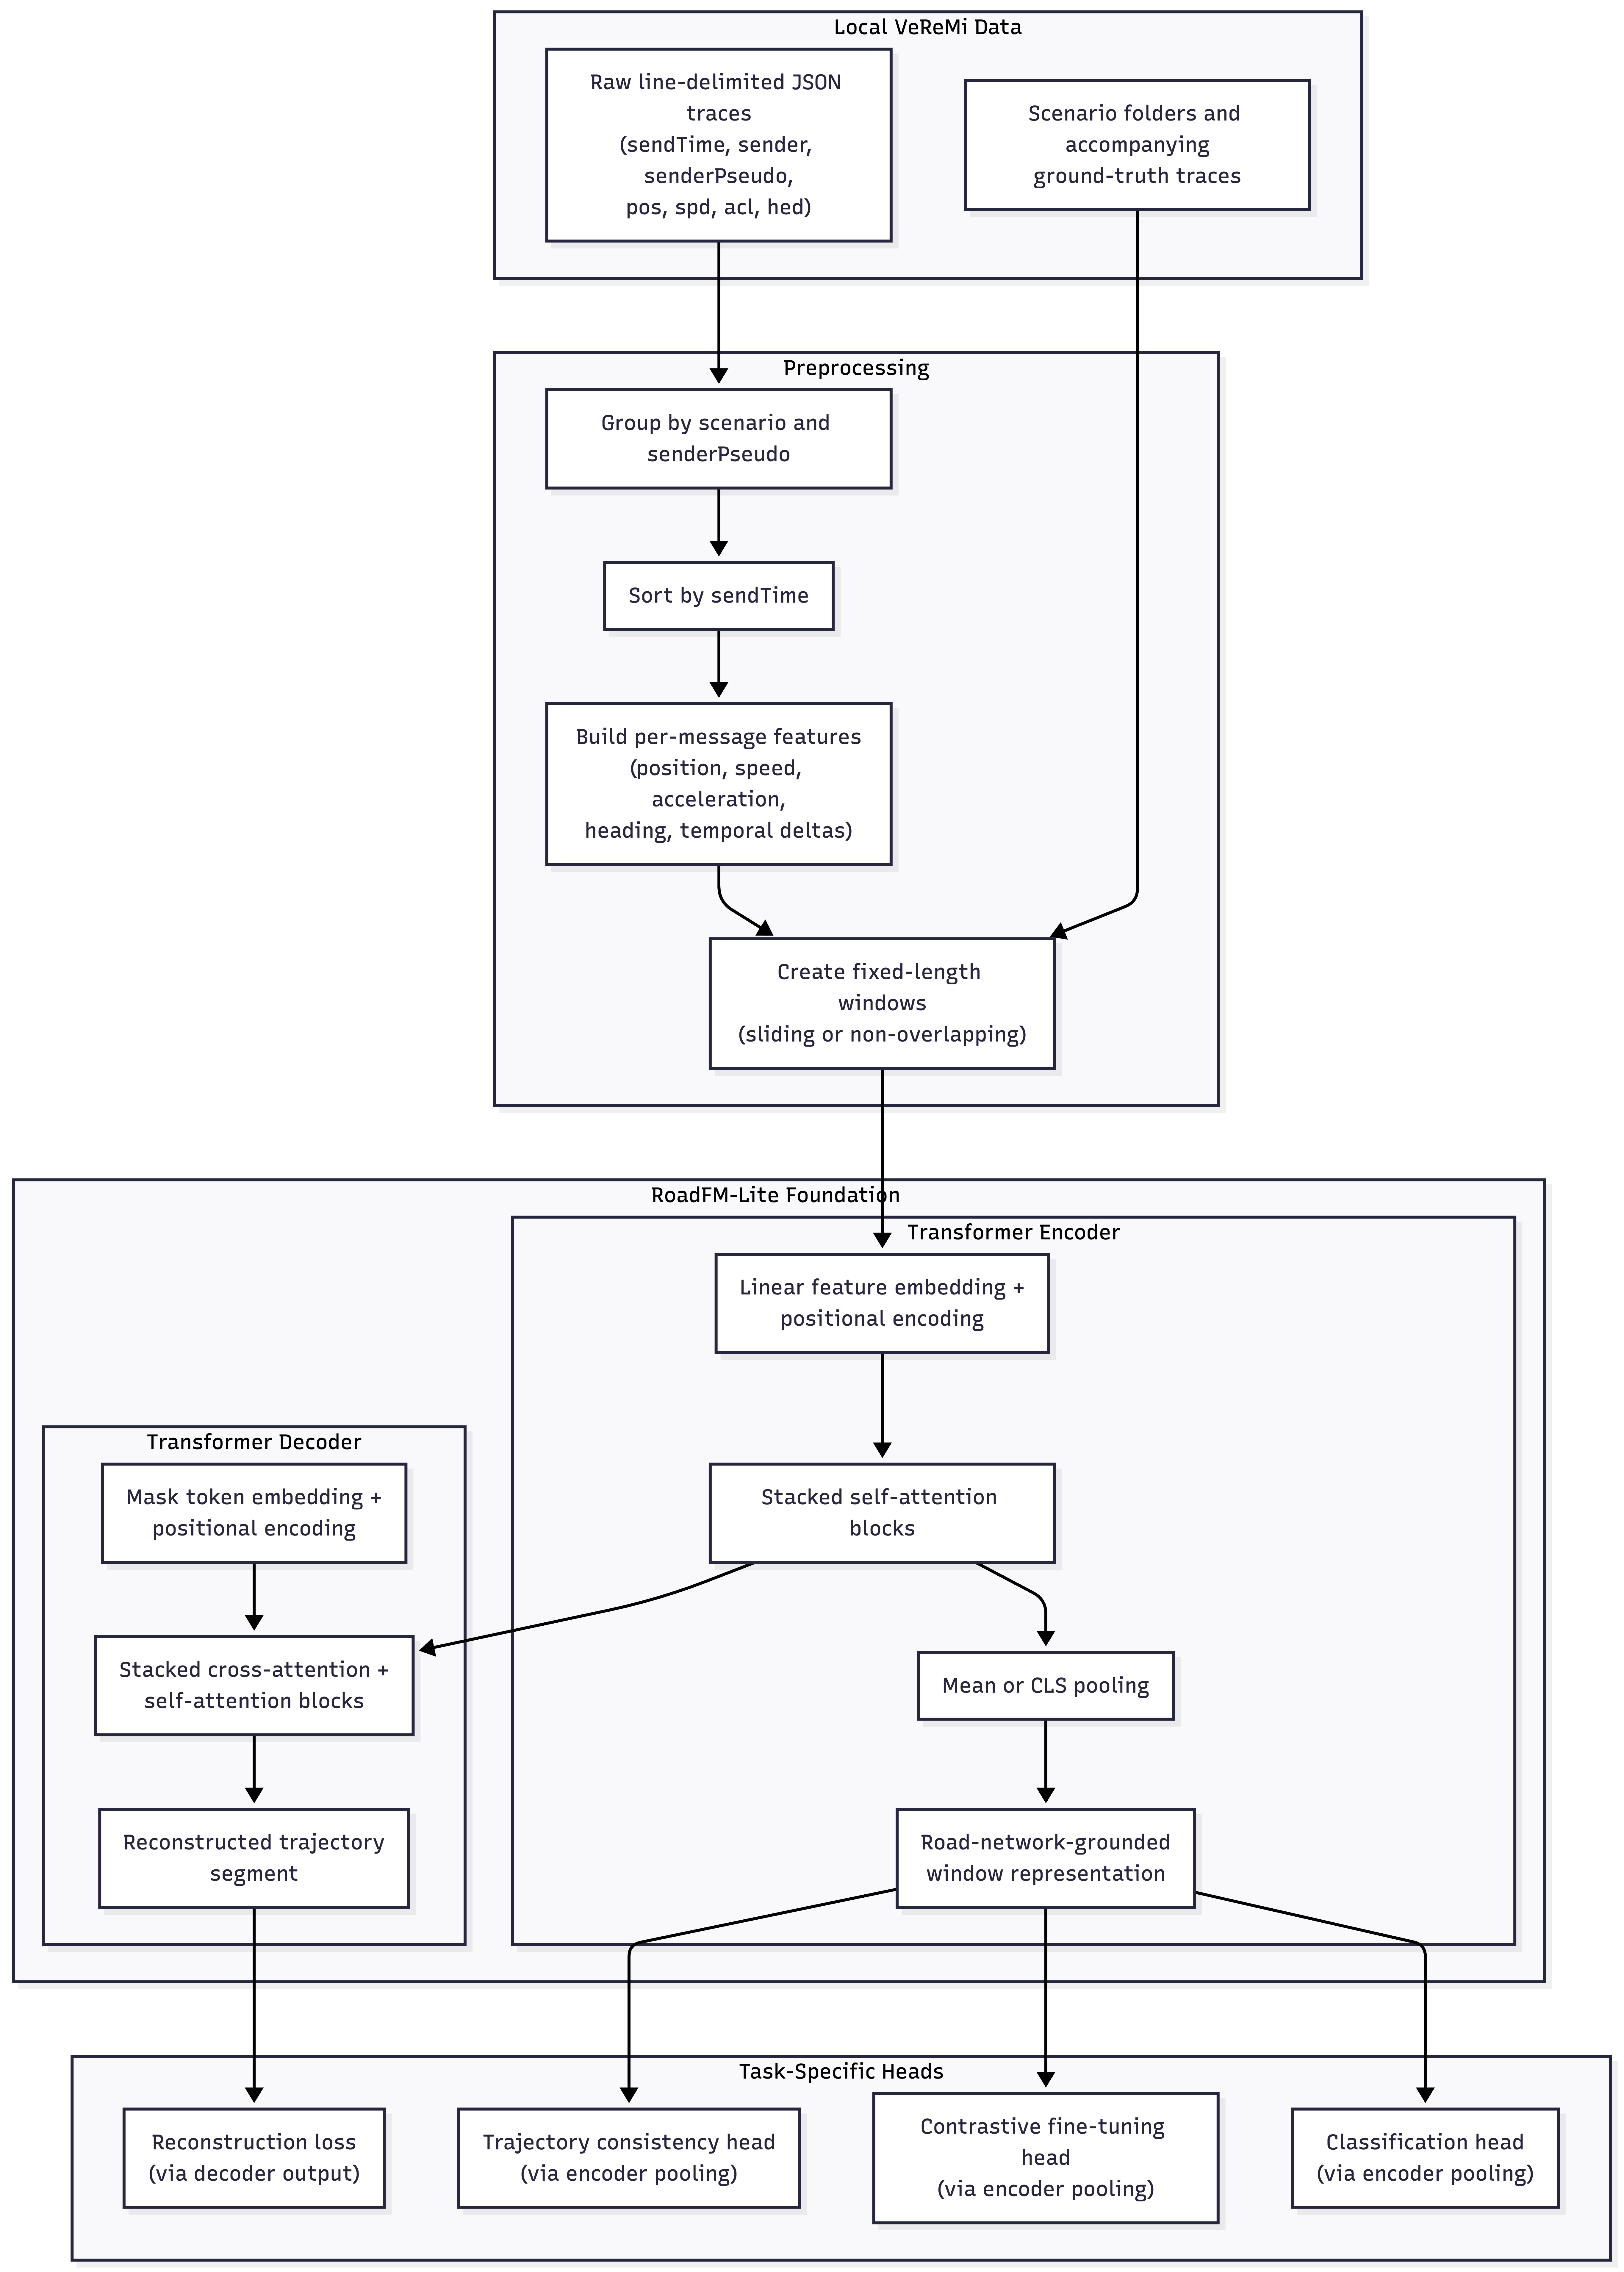
\includegraphics[width=0.88\textwidth,keepaspectratio]{Figures/RoadFMLiteArchitecture.png}
\caption{RoadFM-Lite end-to-end architecture. Preprocessing produces sender-aligned windows; the encoder--decoder foundation model is trained with MTR and TCP; after pretraining, only encoder embeddings are used for few-shot contrastive adaptation, linear classification, or zero-shot retrieval.}
\label{fig:architecture}
\end{figure}

\noindent Figure~\ref{fig:architecture} summarizes the pipeline from raw traces to downstream heads. Subsections~\ref{subsec:window}--\ref{subsec:decoder} formalize window construction, the encoder, and the decoder; Subsection~\ref{subsec:phases} summarizes which components are active in pretraining versus downstream evaluation.

\FloatBarrier

\subsection{VeReMi Window Construction}\label{subsec:window}

Each vehicular message is treated as one time step in a sender-aligned sequence. Let a raw message at time $t$ be
\begin{equation}
m_t = (\mathbf{p}_t, \mathbf{v}_t, \mathbf{a}_t, h_t, \tau_t, u_t),
\end{equation}
where $\mathbf{p}_t$ denotes planar position derived from \texttt{pos}, $\mathbf{v}_t$ denotes planar velocity from \texttt{spd}, $\mathbf{a}_t$ denotes planar acceleration from \texttt{acl}, $h_t$ is heading from \texttt{hed}, $\tau_t$ is the send time, and $u_t$ identifies the sender pseudonym within a scenario.

Messages are grouped first by scenario and sender pseudonym, then sorted by \texttt{sendTime}. Fixed-length windows of length $T$ are created from each ordered sequence. To reduce leakage, split assignment is performed before or jointly with window generation so that overlapping windows from the same source sequence never appear in different partitions.

For each time step, the feature vector $\mathbf{x}_t$ contains the directly observed values plus short-horizon motion deltas:
\begin{equation}
\mathbf{x}_t = [\mathbf{p}_t,\ \mathbf{v}_t,\ \mathbf{a}_t,\ h_t,\ \Delta \tau_t,\ \Delta \mathbf{p}_t,\ \Delta \mathbf{v}_t].
\end{equation}
This representation is intentionally simple. It uses only information present in the dataset while still exposing the encoder to both absolute state and short-term temporal change.

\subsection{Trajectory Encoder}\label{subsec:encoder}

The sequence $\mathbf{X} = \{\mathbf{x}_1, \mathbf{x}_2, \ldots, \mathbf{x}_T\}$ is processed by the Transformer encoder. A linear layer first projects each feature vector into a $d$-dimensional embedding space, sinusoidal positional encoding is added, and the resulting token sequence is passed through $L_e$ stacked self-attention blocks. The encoder outputs contextualized hidden states
\begin{equation}
\mathbf{H} = \{\mathbf{h}_1, \mathbf{h}_2, \ldots, \mathbf{h}_T\} \in \mathbb{R}^{T \times d}.
\end{equation}
The final window-level representation $\mathbf{h}_{\text{win}}$ is obtained either by mean pooling or by a dedicated \texttt{CLS} token prepended to the sequence. For mean pooling,
\begin{equation}
\mathbf{h}_{\text{win}} = \frac{1}{T}\sum_{t=1}^{T} \mathbf{h}_t.
\end{equation}
With a \texttt{CLS} token, $\mathbf{h}_{\text{win}}$ is taken as the corresponding hidden state of that token instead of the average above.

The encoder is the primary output of the foundation model. After pretraining, the encoder representations $\mathbf{H}$ and the pooled embedding $\mathbf{h}_{\text{win}}$ are the artifacts that transfer to all downstream tasks. The encoder is kept compact so that the foundation model remains small enough for repeated few-shot experiments, scenario-holdout studies, and ablations while remaining expressive enough to capture road-network-grounded motion patterns, replay artifacts, temporal irregularities, and motion consistency.

\subsection{Trajectory Decoder}\label{subsec:decoder}

The Transformer decoder is a sequence-to-sequence reconstruction module that learns to recover masked or corrupted trajectory segments by attending to the encoder output. It is used during pretraining and discarded during downstream detection, following the standard encoder-decoder foundation model paradigm (analogous to how BART and T5 drop the decoder for classification tasks).

Given a masked window in which a subset $\mathcal{M}$ of time steps has been replaced by a learned mask token $\mathbf{e}_{\text{mask}}$, the decoder receives the mask token embeddings with positional encoding at the masked positions and attends to the full encoder hidden states $\mathbf{H}$ through cross-attention:
\begin{equation}
\mathbf{D} = \text{TransformerDecoder}(\mathbf{Q}_{\text{mask}},\ \mathbf{H}),
\end{equation}
where $\mathbf{Q}_{\text{mask}} \in \mathbb{R}^{|\mathcal{M}| \times d}$ is the sequence of mask queries with positional information, and $\mathbf{D} \in \mathbb{R}^{|\mathcal{M}| \times d}$ is the decoder output. The decoder consists of $L_d$ layers, each containing masked self-attention over the query sequence, cross-attention to the encoder output, and a feed-forward network.

A linear projection layer then maps each decoder output back to the original feature space:
\begin{equation}
\hat{\mathbf{x}}_t = \mathbf{W}_{\text{rec}} \mathbf{d}_t + \mathbf{b}_{\text{rec}}, \quad t \in \mathcal{M}.
\end{equation}
The decoder serves two purposes in the foundation model. First, it provides a much richer reconstruction signal than a single linear head, because cross-attention allows each masked position to selectively attend to all unmasked encoder representations when predicting the original feature vector. This produces stronger pretraining gradients that propagate back into the encoder, improving the quality of the learned road-network-grounded representations. Second, the decoder makes the foundation model architecturally complete: it supports not only discriminative downstream tasks (via the encoder) but also potential generative tasks such as trajectory prediction, imputation, and anomaly synthesis in future work.

The decoder is deliberately kept lightweight ($L_d \leq L_e$) relative to the encoder, because the thesis prioritizes encoder representation quality for downstream Sybil detection rather than standalone generation capability.

\subsection{Training Phases and Head Separation}\label{subsec:phases}

RoadFM-Lite operates in two distinct phases with different active components:

\textbf{Phase 1: Self-Supervised Pretraining (Encoder + Decoder)}\par\vspace{0.2\baselineskip}
\begin{itemize}
    \item The encoder and decoder are trained jointly.
    \item The decoder reconstructs masked trajectory segments (MTR objective).
    \item The encoder pooling output feeds a consistency classification head (TCP objective).
    \item No labels are used.
\end{itemize}

\textbf{Phase 2: Downstream Detection (Encoder Only)}\par\vspace{0.2\baselineskip}
\begin{itemize}
    \item The decoder is discarded; only the pretrained encoder weights are retained.
    \item A task-specific head is attached to the encoder, depending on the evaluation protocol:
    \begin{itemize}
        \item \textbf{Few-shot:} a projection layer for supervised contrastive fine-tuning on limited labeled samples;
        \item \textbf{Full supervision:} a linear classifier for upper-bound classification;
        \item \textbf{Zero-shot:} no additional head; encoder embeddings are used directly for nearest-neighbor retrieval against a benign memory bank.
    \end{itemize}
\end{itemize}

This separation follows the standard foundation model paradigm: the pretraining phase uses the full encoder-decoder architecture to maximize representation quality, while the downstream phase discards the decoder and evaluates whether the encoder alone has learned transferable structure.

\section{Pretraining Objectives}\label{sec:objectives}

The encoder-decoder foundation model is pretrained on unlabeled trajectory windows using two complementary objectives. Both operate on the same backbone and require no external annotations. The overall pretraining loss is
\begin{equation}
\mathcal{L}_{\text{pretrain}} = \lambda_1 \mathcal{L}_{\text{MTR}} + \lambda_2 \mathcal{L}_{\text{TCP}},
\end{equation}
where $\lambda_1$ and $\lambda_2$ control the balance between reconstruction and consistency learning.

\subsection{Masked Trajectory Reconstruction (MTR)}

Masked trajectory reconstruction teaches the foundation model to infer missing motion from surrounding context using the full encoder-decoder pipeline. Given a window $\mathbf{X} = \{\mathbf{x}_t\}_{t=1}^{T}$, a subset of indices $\mathcal{M}$ is sampled, typically covering 15\% of the time steps. At masked positions, the original token is replaced with a learned mask embedding $\mathbf{e}_{\text{mask}}$ before being fed to the encoder.

The encoder processes the partially masked window and produces contextualized hidden states $\mathbf{H}$. The decoder then takes mask-position queries with positional encoding and attends to $\mathbf{H}$ through cross-attention to reconstruct the original features at masked positions:
\begin{equation}
\mathbf{D} = \text{TransformerDecoder}(\mathbf{Q}_{\text{mask}},\ \mathbf{H}), \quad \hat{\mathbf{x}}_t = \mathbf{W}_{\text{rec}} \mathbf{d}_t + \mathbf{b}_{\text{rec}}, \quad t \in \mathcal{M}.
\end{equation}
The reconstruction loss is the mean squared error over masked positions:
\begin{equation}
\mathcal{L}_{\text{MTR}} = \frac{1}{|\mathcal{M}|} \sum_{t \in \mathcal{M}} \left\|\hat{\mathbf{x}}_t - \mathbf{x}_t\right\|_2^2.
\end{equation}
Using the decoder for reconstruction rather than a simple linear head is important for two reasons. First, cross-attention allows each masked position to selectively gather information from all unmasked encoder states, producing richer reconstruction signals than a per-token linear projection. Second, the reconstruction gradients propagate through both the decoder and back into the encoder via cross-attention, producing stronger encoder representations. This objective encourages the encoder to learn short-horizon motion regularities such as smooth displacement, consistent heading evolution, and reasonable temporal continuity. It is the main mechanism through which the foundation model learns what normal road-network-grounded vehicular trajectories look like without using labels.

\subsection{Trajectory Consistency Prediction (TCP)}

Trajectory consistency prediction trains the encoder to distinguish clean trajectory windows from windows corrupted by synthetic perturbations derived directly from the benchmark. Let $g(\cdot)$ be a corruption operator sampled from a set
\begin{equation}
\mathcal{G} = \{\text{identity},\ \text{replay},\ \text{local-shuffle},\ \text{speed-scale},\ \text{position-offset}\}.
\end{equation}
For each original window $\mathbf{X}$, we generate $\tilde{\mathbf{X}} = g(\mathbf{X})$ and assign a corruption label $c$. The identity operator yields a clean window; the other operators generate controlled inconsistencies that mimic patterns relevant to Sybil behavior:

\begin{itemize}
    \item \textbf{Replay:} Duplicate or reinsert an earlier subsequence into the current window.
    \item \textbf{Local shuffle:} Randomly reorder a short segment while preserving the rest of the window.
    \item \textbf{Speed scale:} Multiply the speed profile and corresponding short-horizon displacement by a factor.
    \item \textbf{Position offset:} Add a persistent offset to position-related components across the window.
\end{itemize}

The encoder produces a window embedding $\mathbf{h}_{\text{win}}$, and a softmax head predicts the corruption class:
\begin{equation}
\hat{\mathbf{y}} = \operatorname{softmax}\!\left(\mathbf{W}_{\text{tcp}}\,\mathbf{h}_{\text{win}} + \mathbf{b}_{\text{tcp}}\right).
\label{eq:tcp_softmax}
\end{equation}
The TCP loss is cross-entropy over corruption classes, with one-hot $y_k$ and predicted probabilities $\hat{y}_k$:
\begin{equation}
\mathcal{L}_{\text{TCP}} = - \sum_{k=1}^{|\mathcal{G}|} y_k \log \hat{y}_k,
\end{equation}
where $\hat{y}_k$ is the $k$-th component of $\hat{\mathbf{y}}$ in \eqref{eq:tcp_softmax}.

TCP is deliberately closer to the downstream problem than a generic augmentation objective. It teaches the encoder to become sensitive to replay artifacts, temporal disorder, and persistent offsets that are plausible manifestations of Sybil-style fabrication in vehicular message traces.

\section{Downstream Task: Sybil Detection}

After pretraining, the decoder and self-supervised heads are discarded and the pretrained encoder is evaluated on Sybil detection tasks built from the same dataset. The central question is whether the road-network-grounded representations learned by the full encoder-decoder foundation model improve downstream discrimination and label efficiency compared to encoder-only training from scratch.

\subsection{Few-Shot Contrastive Fine-Tuning}

In realistic deployments, labeled attack traces are limited. Few-shot contrastive fine-tuning evaluates whether the pretrained encoder can adapt with only a small support set.

\textbf{Setup.} A support set of $K$ labeled windows per class is sampled from the VeReMi training partition, with $K \in \{5, 10, 20\}$. The class set is defined by the locally available scenario families: benign, DataReplaySybil, DoSDisruptiveSybil, DoSRandomSybil, and GridSybil, subject to availability after preprocessing.

\textbf{Supervised Contrastive Loss.} Fine-tuning uses an InfoNCE-style supervised contrastive loss \cite{chen2023self,lin2023pre} to pull same-class trajectory embeddings together while pushing different-class embeddings apart:
\begin{equation}
\mathcal{L}_{\text{InfoNCE}} = -\frac{1}{|B|}\sum_{i \in B} \log \frac{\exp\!\bigl(\text{sim}(\mathbf{h}_i, \mathbf{h}_{j^{+}(i)}) / \tau\bigr)}{\sum_{j \in B \setminus \{i\}} \exp\!\bigl(\text{sim}(\mathbf{h}_i, \mathbf{h}_j) / \tau\bigr)}.
\end{equation}
Here $B$ is the mini-batch, $j^{+}(i)$ indexes a positive pair for anchor $i$ (same class), $\text{sim}(\cdot,\cdot)$ is cosine similarity, and $\tau$ is a temperature.

\textbf{Evaluation.} After fine-tuning, a linear classifier is trained on the learned embeddings. Results are reported both as multiclass family recognition and as binary benign-versus-Sybil detection, with F1 and AUROC serving as the main summary metrics.

\subsection{Zero-Shot Retrieval-Based Detection}

Zero-shot retrieval evaluates whether the pretrained encoder can flag suspicious windows without any labeled attack data, using only benign reference behavior.

\textbf{Memory Bank Construction.} A memory bank $\mathcal{M}_{\text{benign}}$ is populated with embeddings from verified benign trajectory windows in the training partition.

\textbf{Detection Protocol.} For each test window with embedding $\mathbf{h}_{\text{test}}$, the distance to its $k$ nearest benign neighbors is computed:
\begin{equation}
d(\mathbf{h}_{\text{test}}) = \frac{1}{k}\sum_{j=1}^{k} \left\| \mathbf{h}_{\text{test}} - \mathbf{h}_{(j)} \right\|_2
\end{equation}
where $\mathbf{h}_{(j)}$ is the $j$th nearest neighbor in the benign memory bank. A test window is flagged as suspicious when $d(\mathbf{h}_{\text{test}}) > \delta$, with $\delta$ calibrated on validation data.

This setting is important because it tests representation quality directly. If the learned embedding space is meaningful, clean benign windows should cluster while replayed, offset, or otherwise corrupted Sybil windows should fall farther away from the benign reference set.

\subsection{Classification Fine-Tuning}

As an upper-bound reference, the pretrained encoder is also fine-tuned with a standard cross-entropy classifier using the full labeled training split. This setting answers a separate question from few-shot learning: whether self-supervised initialization still helps when all available labels are used.

\section{Baselines}

The proposed model is compared against three baselines that can all be trained using the same inputs and splits.

\subsection{Baseline 1: Same Encoder From Scratch}

This is the primary controlled baseline. It uses the exact same encoder architecture and input features as RoadFM-Lite but removes the encoder-decoder pretraining phase entirely. The encoder is initialized randomly and trained directly on the downstream labels only.

This comparison isolates the value of the foundation model's self-supervised pretraining. If the pretrained encoder outperforms this baseline, the improvement cannot be attributed to extra input features or a larger architecture, but to the representations learned through the encoder-decoder pretraining process.

\subsection{Baseline 2: Feature Engineering + Random Forest}

This baseline represents the traditional non-deep-learning approach. Each window is summarized by hand-crafted kinematic features and classified with a Random Forest. The feature set includes speed statistics, acceleration statistics, heading statistics, displacement statistics, temporal statistics, and motion smoothness summaries as described in the proposal draft.

This baseline provides a practical benchmark for how far simple, interpretable summary features can go on this dataset without sequence pretraining.

\subsection{Baseline 3: Supervised BiLSTM Sequence Classifier}

This baseline feeds the same feature sequence into a standard bidirectional LSTM followed by a classification head. It tests whether the benefits of RoadFM-Lite come from self-supervised pretraining rather than from sequence modeling alone.

\section{Evaluation Plan}

The evaluation methodology is designed to assess four properties of the learned representation: detection quality, label efficiency, scenario robustness, and component contribution.

\subsection{Detection Metrics}

All detection experiments report precision, recall, F1-score, and AUROC on held-out test data. Metrics are reported for both binary benign-versus-Sybil detection and per-family analysis across the available attack families.

\begin{table}[H]
\centering
\small
\begin{singlespace}
\begin{tabularx}{\textwidth}{@{}>{\RaggedRight\arraybackslash}p{1.6cm}>{\RaggedRight\arraybackslash}p{3.35cm}>{\RaggedRight\arraybackslash}X@{}}
\toprule
\textbf{Metric} & \textbf{Definition} & \textbf{Purpose} \\
\midrule
Precision & $\mathrm{TP}/(\mathrm{TP}+\mathrm{FP})$ & Penalizes false alarms on legitimate vehicles \\
Recall & $\mathrm{TP}/(\mathrm{TP}+\mathrm{FN})$ & Measures coverage of Sybil identities \\
F1-score & Harmonic mean of precision and recall & Balanced operating point \\
AUROC & Area under the ROC curve & Threshold-free separability \\
\bottomrule
\end{tabularx}
\end{singlespace}
\caption{\textbf{Primary detection metrics.} Definitions and roles used for all evaluation experiments.}
\label{tab:detection_metrics}
\end{table}

\subsection{Leakage-Safe Split Protocol}

Because trajectory windows are extracted from continuous traces, preventing leakage is essential. The split protocol follows three rules: (1) partition at the scenario-group and sender-sequence level before creating overlapping windows whenever possible; (2) keep all windows derived from the same source subsequence in exactly one split; (3) compute normalization statistics on the training partition only.

\subsection{Few-Shot Analysis Protocol}

The few-shot evaluation measures label efficiency. From the VeReMi training split, sample $K$ labeled windows per class for $K \in \{5, 10, 20\}$, fine-tune with supervised contrastive loss, evaluate on the full held-out test split, and repeat each $K$-shot experiment five times with different random support sets to report mean and standard deviation.

\subsection{Scenario-Holdout Generalization}

Train on the \texttt{0709} scenario groups and evaluate on \texttt{1416}, then swap roles. Report the same metrics used in the standard split setting. Optionally extend with attack-family holdout. The holdout degradation is
\begin{equation}
\Delta_{\text{scenario}} = \frac{\text{F1}_{\text{standard}} - \text{F1}_{\text{holdout}}}{\text{F1}_{\text{standard}}} \times 100\%.
\end{equation}

\subsection{Ablation Study}

Ablations remove MTR, TCP, the decoder, delta features, or vary window length; each variant is evaluated under the same few-shot protocol ($K = 10$) and the full-supervision setting, reporting at least F1 and AUROC.

\subsection{Additional Analyses}

Results will be reported per attack family where applicable, with qualitative error analysis for false positives and false negatives.

\section{Dataset Scope and Preprocessing}

\begingroup
\setlength{\intextsep}{4pt plus 2pt minus 2pt}
\setlength{\textfloatsep}{6pt plus 3pt minus 3pt}
\setlength{\floatsep}{6pt plus 3pt minus 3pt}
\captionsetup{skip=4pt}

This thesis uses only the local VeReMi Sybil dataset available in the workspace. No external trajectory corpora, road-network assets, or additional simulators are required.

\begin{figure}[H]
\centering
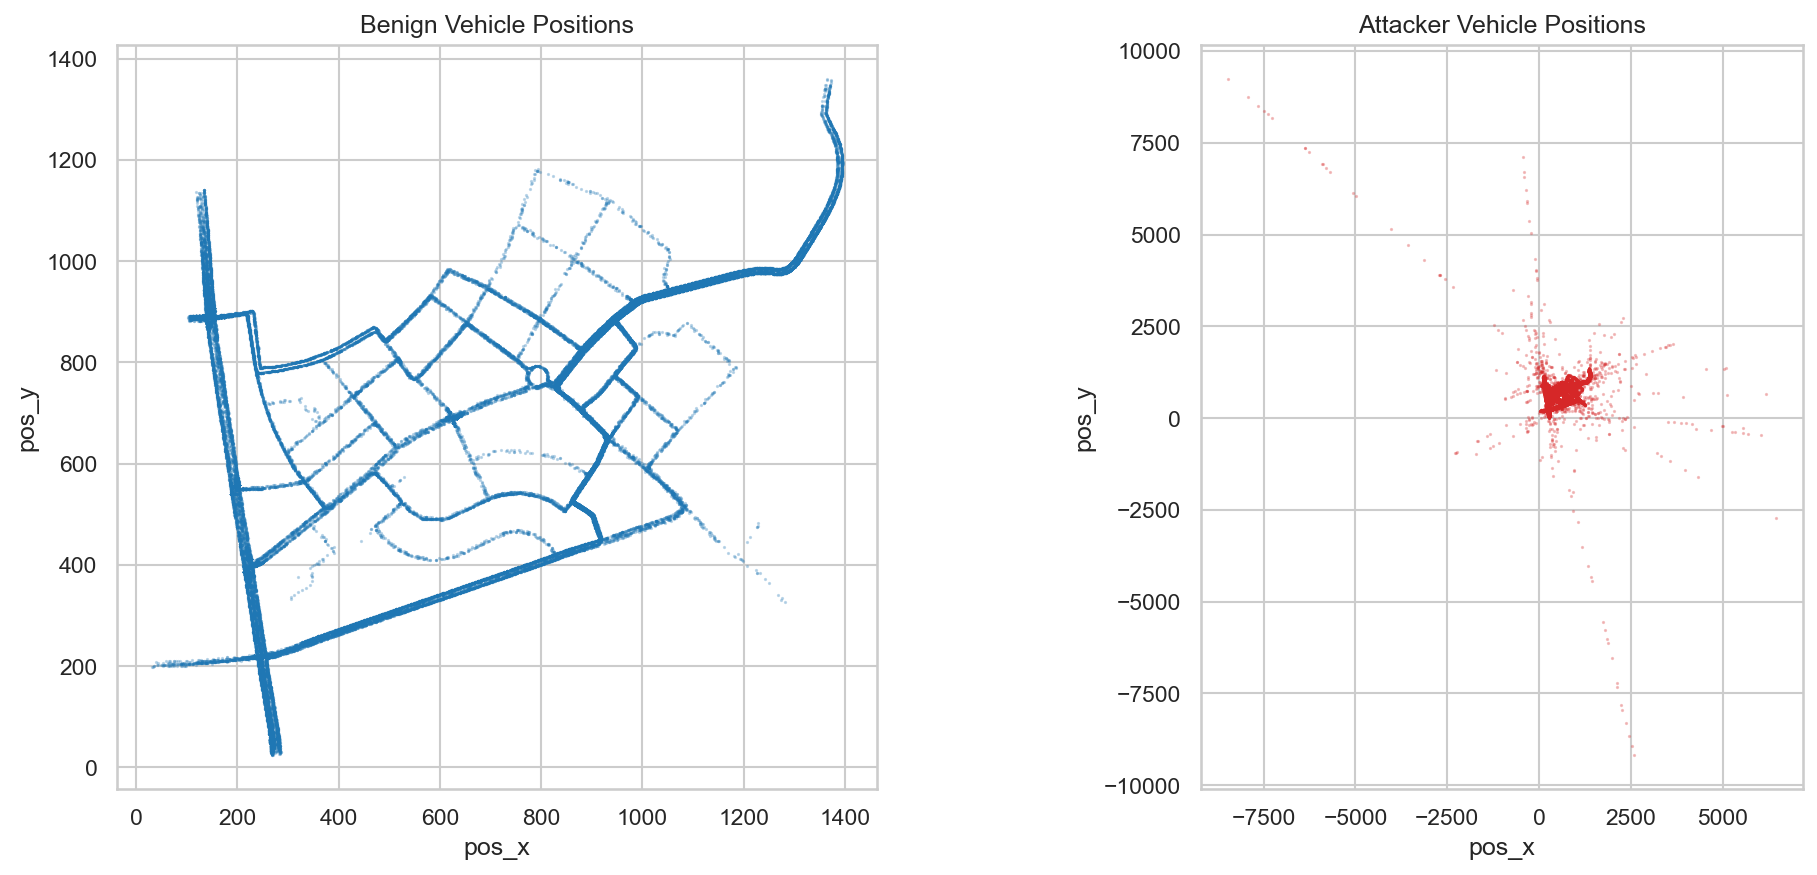
\includegraphics[width=0.96\textwidth,keepaspectratio]{Figures/fig_spatial_coverage.png}
\caption{Exploratory spatial coverage of sampled VeReMi traces: benign and attacker positions in the simulation frame (geographic spread and co-location for windowing).}
\label{fig:eda_spatial}
\end{figure}

\noindent Figure~\ref{fig:eda_spatial} gives a concrete sense of how vehicles populate the urban grid before split construction and window extraction.

\begin{figure}[H]
\centering
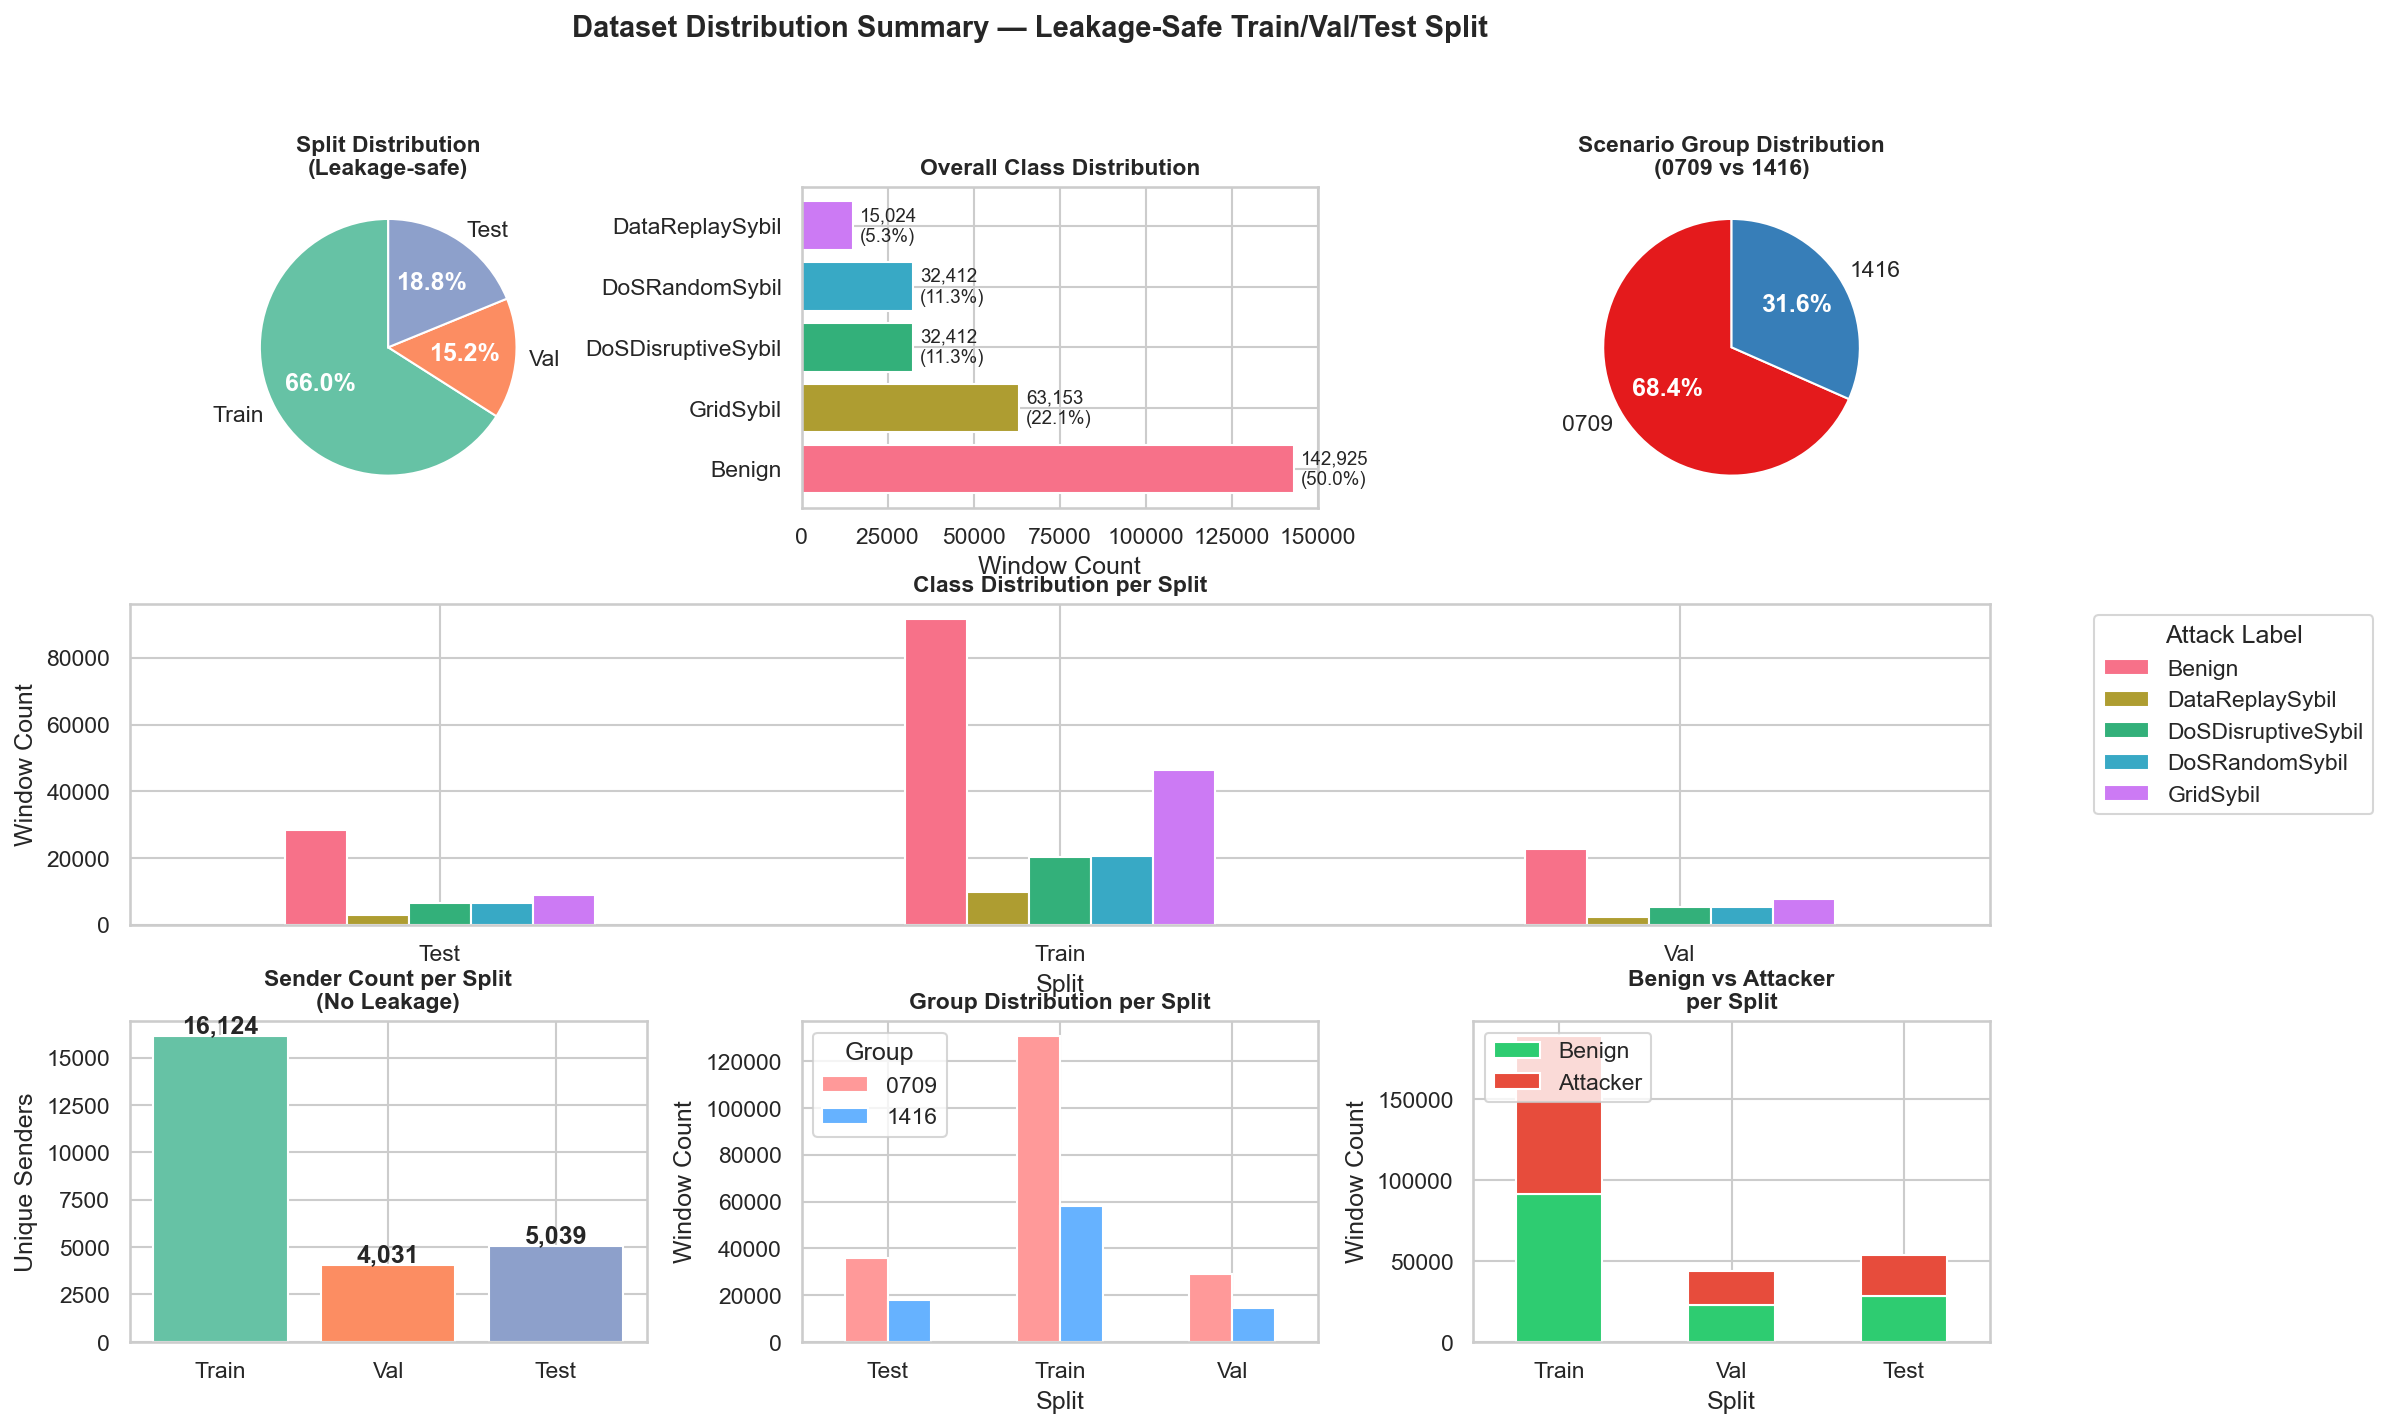
\includegraphics[width=0.96\textwidth,keepaspectratio]{Figures/fig_dataset_distribution.png}
\caption{Dataset distribution summary: leakage-safe splits, class and scenario-group counts, per-split sender counts, and benign vs.\ attacker balance.}
\label{fig:dataset_distribution}
\end{figure}

\noindent Figure~\ref{fig:dataset_distribution} expands on this overview: sender-disjoint train/val/test partitions; overall window counts for benign vs.\ the four Sybil families; mix of scenario groups \texttt{0709} and \texttt{1416}; per-split class histograms; unique senders per split; and benign vs.\ attacker ratios.
These statistics align with the training and evaluation splits described in this section.

\subsection{Local Scenario Coverage}

The available data is organized into VeReMi scenario families including DataReplaySybil, DoSDisruptiveSybil, DoSRandomSybil, and GridSybil, each with local groups \texttt{0709} and \texttt{1416} for pretraining and downstream evaluation. Within each family and group folder, time-windowed VeReMi subdirectories contain line-delimited trace files and accompanying ground-truth traces.

\subsection{Available Message Fields}

Each message trace includes at minimum \texttt{sendTime}, \texttt{sender}, \texttt{senderPseudo}, \texttt{pos}, \texttt{spd}, \texttt{acl}, and \texttt{hed}. Noise-augmented variants may be present but the core proposal uses the main kinematic fields.

\subsection{Window Generation and Label Use}

For self-supervised pretraining, labels are ignored. For downstream evaluation, labels are derived from the scenario family and ground-truth trace organization. For benign reference retrieval, only benign windows from the training split populate the memory bank.

\subsection{Road-Network Grounding and Dataset Scope}

The VeReMi dataset supports learning road-network-grounded trajectory representations because it is generated by SUMO on a detailed urban road network. Focusing the thesis on this benchmark supports reproducibility and a concrete contribution within a master's timeline.

\endgroup
\FloatBarrier

\section{Timeline and Deliverables}

The thesis is structured across two semesters with systematic progression from data preparation through implementation, evaluation, and thesis writing. The timeline emphasizes implementation work and thesis development, while still including few-shot and zero-shot studies as secondary validation tracks.

\subsection{Detailed Timeline Overview}

\begin{table}[H]
\centering
\small
\setlength{\tabcolsep}{6pt}
\renewcommand{\arraystretch}{1.4}
\begin{tabularx}{\textwidth}{|>{\RaggedRight\arraybackslash}p{2.35cm}|>{\RaggedRight\arraybackslash}X|>{\RaggedRight\arraybackslash}X|}
\hline
\textbf{Phase (Months)} & \textbf{Research \& Writing} & \textbf{Implementation \& Development} \\[0.5\baselineskip]\hline\hline
\textbf{Aug--Sep 2026} (1--2) & Literature review; architecture design; methodology finalization & GPU setup; dataset exploration; preprocessing pipeline \\[0.5\baselineskip]\hline
\textbf{Oct--Dec 2026} (3--5) & Pretraining objectives; evaluation framework design; baseline docs & Encoder--decoder implementation; MTR/TCP modules; pipeline integration \\[0.5\baselineskip]\hline
\textbf{Jan--Feb 2027} (6--7) & Experiments execution; results analysis; draft Methods/Dataset & Full pretraining run; downstream heads; contrastive modules \\[0.5\baselineskip]\hline
\textbf{Mar--Apr 2027} (8--9) & Results finalization; complete thesis writing; final documentation & Few-shot/zero-shot evaluation; scenario holdout; ablation studies \\[0.5\baselineskip]\hline
\end{tabularx}
\caption{\textbf{Thesis development timeline.} Parallel research and implementation phases spanning 9 months (Aug 2026 -- Apr 2027).}
\label{tab:timeline}
\end{table}

Expected contributions include: (1) a road-network-grounded trajectory foundation model pipeline; (2) empirical validation for data-efficient Sybil detection; and (3) a benchmark-centered scenario-holdout evaluation protocol with reproducible split definitions.

Success criteria include competitive or improved F1 and AUROC versus the from-scratch encoder under full supervision, measurable advantage in at least one low-label setting $K \in \{5, 10, 20\}$, and lower scenario-holdout degradation than the from-scratch baseline, supported by ablation evidence for MTR, TCP, and window design.

\subsection{Connection to Sybil Guard Project}

This thesis produces a pretrained trajectory foundation model relevant to downstream security experiments, with reusable weights and preprocessing, few-shot validation, scenario-holdout robustness, and a compact encoder suitable for future federated or personalized detection pipelines.

\clearpage
\begingroup
\renewcommand{\refname}{REFERENCES}
\singlespacing
\setlength{\parskip}{0.18em}
\bibliographystyle{IEEEtran}
\bibliography{references}
\endgroup

\end{document}
